\chapter{Strumenti utilizzati}\label{ch:capitolo2}
\section{Realtà virtuale}
Il concetto di realtà virtuale non è recente come si possa pensare, le prime testimonianze risalgono al 1960 con la \textit{Telesphere Mask}, brevettata da Heiling, che era stata pensata come un apparato da collegare alla tv per simulare la sensazione di realtà muovendosi nelle tre dimensioni. Allora però non ebbe il successo sperato, il boom di questa tecnologia è arrivato solo nel 2012 con l'uscita dell'\textit{Oculus Rift} che la ha resa accessibile a milioni di utenti in tutto il mondo.\\\\
Una definizione ufficiale di realtà virtuale non esiste ancora, le più accreditate sono però quella data da Isdale nel 1998 "È la simulazione di un ambiente reale o immaginario che può essere sperimentato visivamente nelle tre dimensioni e che fornisce inoltre un'esperienza interattiva con il suono e possibilmente anche con feedback tattili o di altre forme. La realtà virtuale è un modo per gli esseri umani di visualizzare, manipolare e interagire con computer e dati estremamente complessi" e quella data da Baieier nel 1993 "È un ambiente artificiale creato con hardware e software di computer e presentato a un utente in modo tale che appaia e si senta come un ambiente reale", pertanto la realtà virtuale si riferisce a un mondo 3D completamente immersivo e interattivo creato con l'utilizzo di un calcolatore che permette all'utente, grazie all'uso di un Head Mounted Display, di entrarvi e di diventare parte attiva di esso \cite{inbook}.\\\\
L'architettura necessaria per far funzionare il tutto si compone di un visore con un campo visivo dai 100 ai 110 gradi e un frame rate compreso tra 60fps e 120fps dotato anche di sensori che permettono, insieme ad almeno due \textit{base station}, l'\textit{Head Tracking} ovvero lo spostamento dell'immagine in base alla posizione della testa. Per poter interagire effettivamente con il mondo circostante vengono utilizzati due controller, uno per mano, sempre rilevati dalle \textit{base station}.\\\\
Spesso il concetto realtà virtuale viene confuso con quello di realtà aumentata; quest'ultima però è un potenziamento della percezione del mondo reale al quale vengono aggiunti dei contenuti digitali e che non necessita di hardware appositi per funzionare ma può essere applicata anche con l'utilizzo di smartphone o tablet. Un classico esempio di realtà aumentata è un famoso gioco Nintendo uscito nel 2016, \textit{Pokemon Go}, nel quale i personaggi venivano proiettati nel mondo reale e il giocatore poteva interagire con loro e catturarli. \\\\
Anche se attualmente l'applicazione principale di questa tecnologia è nel campo videoludico ultimamente sta trovando spazio anche in altri campi come ad esempio quello dell'addestramento militare. \textit{DoDAAM}, un azienda coreana, ha già creato tutta una serie di simulazioni di situazioni di guerra come ad esempio il lancio da un aeroplano, la guida di un carro armato e di un jet riducendo contemporaneamente costi, tempi e rischi. Altre applicazioni si possono trovare nel ambito medico sopratutto nella terapia di disturbi psichiatrici e nella riabilitazione motoria e cognitiva. Le potenzialità della realtà virtuale possono essere usate anche nella formazione del personale medico simulando, ad esempio, un operazione chirurgica.	
\subsection{Htc Vive Pro}
\begin{figure}[h!]
	\centering
	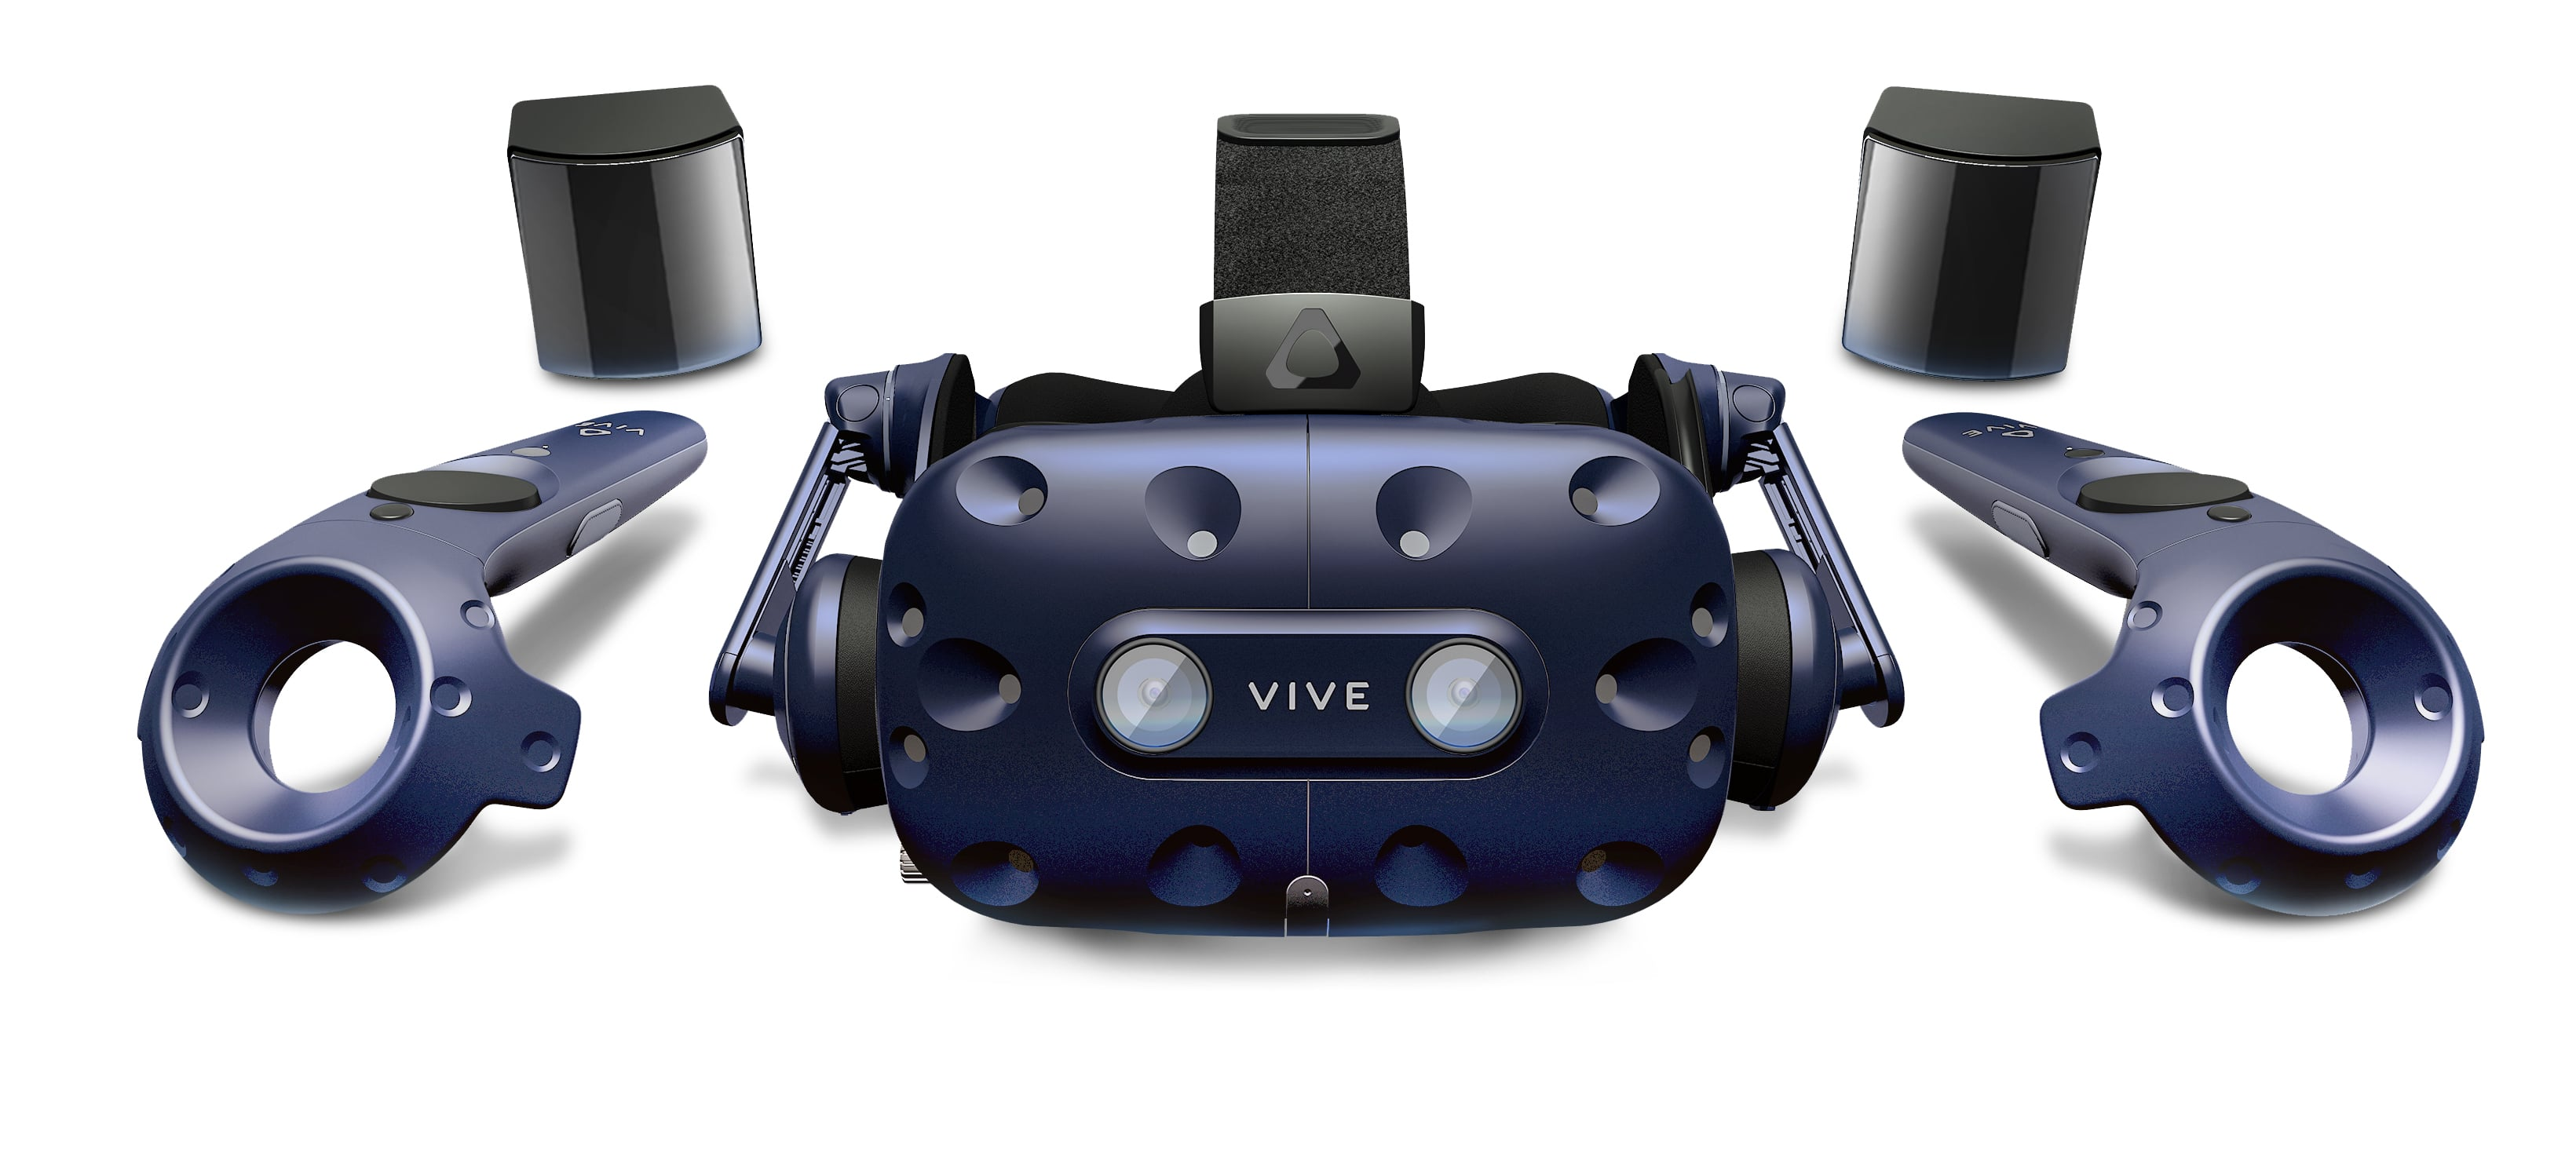
\includegraphics[width=1\linewidth]{../immagini/vive}
	\caption[Htc Vive]{Visore e componenti }
	\label{fig:vive}
\end{figure}
Il sistema di realtà virtuale utilizzato durante la realizzazione del progetto è l'HTC Vive Pro, prodotto da HTC e Valve, (in Figura 2.1) e commercializzato a partire dal 2016. Il visore VIVE presenta due lenti Fresnel non perfettamente circolari ma con un lato piatto che le allinea con il naso permettendo anche di avvicinarle o allontanarle tra loro permettendo di adattarle alla propria distanza interpupillare. L'HMD presenta oltre ai 32 sensori infrarossi per il tracking posizionati sulla superficie anche un giroscopio, un accelerometro e un sensore di posizione laser per riprodurre nella maniera più fedele possibile il movimento della testa.\\
I \textit{controller} servono per interagire con l'ambiente e sono dotati di 24 sensori per il tracking oltre che a una serie di tasti.\\
Le \textit{Base Station} sono degli emettitori, generano una luce ad infrarossi e due fasci laser che vengono rilevati dai sensori posti su controller e HMD. Basandosi poi sulla posizione di questi sensori e su quanto sono stati irradiati è possibile stimare con un ottima precisione la posizione e l'orientamento degli oggetti rispetto alle base station.\\\\
Per la configurazione di questo strumento ci si avvale di un runtime chiamato \textit{SteamVR} ncluso nel client di Steam che consente di usufruire della realtà virtuale. SteamVR viene installato automaticamente quando Steam rileva la connessione di un visore al PC dell'utente, ma può essere installato anche manualmente.\\
SteamVR consente all'utente la gestione di molti aspetti della sua esperienza di gioco tra cui:
\begin{itemize}
	\item Configurazione della stanza, con cui definire la propria area di gioco.
	\item Controllo stato e gestione del dispositivo, con cui aggiornare il firmware, associare nuovi dispositivi, cambiare le impostazioni audio, impostare la duplicazione e personalizzare funzionalità quali il Motion Smoothing \cite{steamvr}.
\end{itemize}
Attualmente è uno dei migliori dispositivi disponibili sul mercato e come tale per funzionare il pc su cui far girare il tutto deve soddisfare alcuni requisiti. Di seguito vengono riportati quelli consigliati presi direttamente dal sito ufficiale della Vive:
\begin{itemize}
	\item \textbf{Processore} Intel Core i5 o superiore
	\item \textbf{GPU} NVIDIA GeForce GTX 1070/Quadro P5000, AMD Radeon Vega 56 o superiore
	\item \textbf{Memoria} 4Gb di RAM o più
	\item \textbf{Video Output} DisplayPort 1.2 o più recente
	\item \textbf{USB port} 1x USB 3.0 o più recente
	\item \textbf{O.S.} Windows 10
\end{itemize} 

\section{Unity 3D}
Unity è un motore grafico sviluppato da Unity Technologies usato principalmente per sviluppare videogiochi e simulazioni in grafica 2D o 3D tramite scripting in C\#. È un ambiente multi-piattaforma che permette la creazione di applicazioni per diversi dispositivi tra cui: Android, iOS, Windows, Playstation e sviluppo di software di realtà virtuale e aumentata. Unity nel suo Asset Store mette a disposizione tutta una serie di librerie, modelli, prefab e script sia gratuiti che a pagamento. Tra questi nel progetto viene utilizzato OpenVR ovvero un API che consente alle applicazioni di interagire con gli hardware di diversi produttori senza necessità di rilevare l'effettivo hardware puntato. Supporta diversi HMD tra cui Valve Index, HTC Vive, Oculus Rift, Windows Mixed Reality e altri.
\section{Blender}
Blender è una suite di creazione 3D gratuita e open source. Il software mette a disposizione diverse funzionalità tra cui modellazione 3D, texuring, simulazione di elementi come corpi rigidi, fluidi e fumi, animazione 3D, rendering ecc.\\
Nel progetto servirà per la gestione di tutti i dati 3D in particolare per la fase di pre-process per creare la scena e nella fase di post-process per visualizzare e maneggiare i risultati. 
\subsection{Modelli 3D} 
\begin{figure}
	\centering
	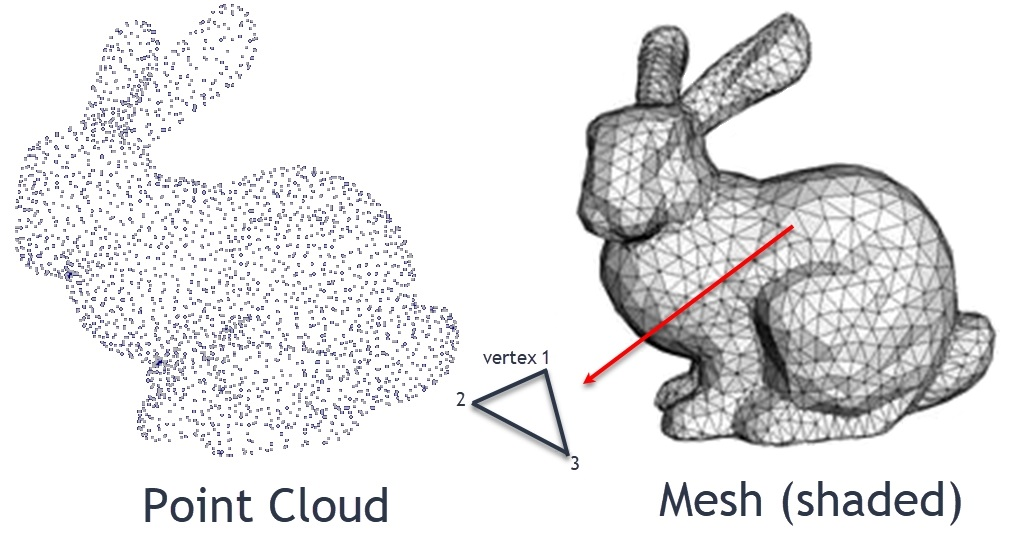
\includegraphics[width=0.8\linewidth]{../immagini/meshpoint}
	\caption[Mesh e Pointcloud]{Esempio di mesh e pointcloud }
	\label{fig:meshpoint}
\end{figure}
Tra i vari modelli 3D che si possono trovare nella computer grafica e che durante la realizzazione del progetto sono stati particolarmente ricorrenti troviamo \textit{mesh} e \textit{poitncloud}.\\
Una mesh poligonale, detta anche maglia poligonale, è una collezione di vertici, spigoli e facce che definiscono la forma di un oggetto poliedrico. . Le facce consistono, di
solito, di rettangoli, triangoli, o altri semplici
poligoni convessi, dal momento che ci`o
semplifica il rendering.\\
Una mesh poligonale si compone di tre tipi di elementi:
\begin{itemize}
	\item Il \textbf{vertice} è una posizione nello spazio e ha
	informazioni relative al colore e al vettore normale.
	\item Il \textbf{lato} è il collegamento tra due vertici.
	\item La \textbf{faccia} un insieme chiuso di lati, ad esempio una faccia triangolare avrà tre lati e una faccia quadrangolare avrà quattro lati. Un poligono è un insieme complanare di facce. Ogni faccia ha inoltre anche un vettore normale alla sua superficie. 
\end{itemize}
Una point cloud, invece, è un insieme di punti nello spazio non dotato di informazioni topologiche (niente lati ne triangoli), questo tipo di dati proviene dall'utilizzo di scanner 3D o sensori come il Kinect.  	 

